\documentclass[12pt,halfline,a4paper,]{ouparticle}

% Packages I think are necessary for basic Rmarkdown functionality
\usepackage{hyperref}
\usepackage{graphicx}
\usepackage{listings}
\usepackage{color}
\usepackage{fancyvrb}
\usepackage{framed}

%% To allow better options for figure placement
%\usepackage{float}

% Packages that are supposedly required by OUP sty file
\usepackage{amssymb, amsmath, geometry, amsfonts, verbatim, endnotes, setspace}

% For code highlighting I think
\DefineVerbatimEnvironment{Highlighting}{Verbatim}{commandchars=\\\{\}}
\definecolor{shadecolor}{RGB}{248,248,248}
\newenvironment{Shaded}{\begin{snugshade}}{\end{snugshade}}
\newcommand{\AlertTok}[1]{\textcolor[rgb]{0.94,0.16,0.16}{#1}}
\newcommand{\AnnotationTok}[1]{\textcolor[rgb]{0.56,0.35,0.01}{\textbf{\textit{#1}}}}
\newcommand{\AttributeTok}[1]{\textcolor[rgb]{0.77,0.63,0.00}{#1}}
\newcommand{\BaseNTok}[1]{\textcolor[rgb]{0.00,0.00,0.81}{#1}}
\newcommand{\BuiltInTok}[1]{#1}
\newcommand{\CharTok}[1]{\textcolor[rgb]{0.31,0.60,0.02}{#1}}
\newcommand{\CommentTok}[1]{\textcolor[rgb]{0.56,0.35,0.01}{\textit{#1}}}
\newcommand{\CommentVarTok}[1]{\textcolor[rgb]{0.56,0.35,0.01}{\textbf{\textit{#1}}}}
\newcommand{\ConstantTok}[1]{\textcolor[rgb]{0.00,0.00,0.00}{#1}}
\newcommand{\ControlFlowTok}[1]{\textcolor[rgb]{0.13,0.29,0.53}{\textbf{#1}}}
\newcommand{\DataTypeTok}[1]{\textcolor[rgb]{0.13,0.29,0.53}{#1}}
\newcommand{\DecValTok}[1]{\textcolor[rgb]{0.00,0.00,0.81}{#1}}
\newcommand{\DocumentationTok}[1]{\textcolor[rgb]{0.56,0.35,0.01}{\textbf{\textit{#1}}}}
\newcommand{\ErrorTok}[1]{\textcolor[rgb]{0.64,0.00,0.00}{\textbf{#1}}}
\newcommand{\ExtensionTok}[1]{#1}
\newcommand{\FloatTok}[1]{\textcolor[rgb]{0.00,0.00,0.81}{#1}}
\newcommand{\FunctionTok}[1]{\textcolor[rgb]{0.00,0.00,0.00}{#1}}
\newcommand{\ImportTok}[1]{#1}
\newcommand{\InformationTok}[1]{\textcolor[rgb]{0.56,0.35,0.01}{\textbf{\textit{#1}}}}
\newcommand{\KeywordTok}[1]{\textcolor[rgb]{0.13,0.29,0.53}{\textbf{#1}}}
\newcommand{\NormalTok}[1]{#1}
\newcommand{\OperatorTok}[1]{\textcolor[rgb]{0.81,0.36,0.00}{\textbf{#1}}}
\newcommand{\OtherTok}[1]{\textcolor[rgb]{0.56,0.35,0.01}{#1}}
\newcommand{\PreprocessorTok}[1]{\textcolor[rgb]{0.56,0.35,0.01}{\textit{#1}}}
\newcommand{\RegionMarkerTok}[1]{#1}
\newcommand{\SpecialCharTok}[1]{\textcolor[rgb]{0.00,0.00,0.00}{#1}}
\newcommand{\SpecialStringTok}[1]{\textcolor[rgb]{0.31,0.60,0.02}{#1}}
\newcommand{\StringTok}[1]{\textcolor[rgb]{0.31,0.60,0.02}{#1}}
\newcommand{\VariableTok}[1]{\textcolor[rgb]{0.00,0.00,0.00}{#1}}
\newcommand{\VerbatimStringTok}[1]{\textcolor[rgb]{0.31,0.60,0.02}{#1}}
\newcommand{\WarningTok}[1]{\textcolor[rgb]{0.56,0.35,0.01}{\textbf{\textit{#1}}}}

% For making Rmarkdown lists
\providecommand{\tightlist}{%
  \setlength{\itemsep}{0pt}\setlength{\parskip}{0pt}}


% Part for setting citation format package: natbib
\usepackage{natbib}
\bibliographystyle{plainnat}

% Part for setting citation format package: biblatex

% Pandoc header

\begin{document}

\title{covid19census: U.S. and Italy COVID-19 epidemiolagical data with
demographic and health related metrics}

\author{%
\name{Claudio Zanettini}\address{Department of Oncology, Johns Hopkins University School of Medicine,
Baltimore, MD, USA}\email{\href{mailto:claudio.zanettini@gmail.com}{claudio.zanettini@gmail.com}}
\and
\name{Luigi Marchionni}\address{Department of Oncology, Johns Hopkins University School of Medicine,
Baltimore, MD, USA}\email{\href{mailto:marchion@jhu.edu}{marchion@jhu.edu}}\thanks{Corresponding author; Email: \href{mailto:marchion@jhu.edu}{marchion@jhu.edu}}
\and
\name{Others to be add}\address{Another University}\email{\href{mailto:otherstobeadd@example.com}{otherstobeadd@example.com}}
}

\abstract{The R package \texttt{covid19census} provides funcions to extract U.S.
and Italy COVID-19 epidemiological data (at the regional and county
level, respectively) and combine the results with relevant demographic
and health related metrics obtained from other sources. The aim of the
packages is to promote and facilitate modeling and analysis of COVID-19
data by the scientific community.}

\date{\today}

\keywords{COVID-19; R}

\maketitle



\hypertarget{introduction}{%
\section{Introduction}\label{introduction}}

In the mist of a virus pandemic, unraveling the constant flow of
epidemiological data is of paramount importance, not only to guide the
evaluation and implementation of non-pharmacological interventions
(NPI), but also to optimize drug development.

For example, in early phases of the pandemic, analysis and modeling of
COVID-19 confirmed cases and deaths has been employed to assess the
effects of NPI in China and Europe \citep{flaxman2020, prem2020tlph}.
More recently, the increased flow of COVID-19 data, and the integration
of different sources of information (seasonality of other coronoviruses,
U.S. clinical care) has allowed even more long-term predictions of the
feasibility and effectiveness of possible containment strategies
\citep{kissler2020s}.

Similarly, early evidences of the correlation between Bacille
Calmette-Guérin vaccination and COVID-19 outcomes spur several clinical
investigations {[}\citet{miller2020m}; \citet{shet2020m};
\href{https://www.who.int/news-room/commentaries/detail/bacille-calmette-gu\%C3\%A9rin-(bcg)-vaccination-and-covid-19}{WHO}{]}.
However, the implications and conclusions of that initial observation
were curtailed by subsequent models that included more factors
\citep[e.s. age;][]{fukui2020m}. Overall, these few examples underscore
the importance in general, of providing public access to ongoing
COVID-19 metrics and in particular, of including multiple heterogeneous
collections of data in modeling and analysis in order to improve
predictions and ultimately, to address the many challenges of the
current pandemic emergency.

The current \texttt{R} package provides tools to rapidly extract United
States and Italy COVID-19 epidemiological metrics (at county and
regional level, respectively) from different sources, and to combine
them with other demographic and health related datasets. The goal of the
package is to facilitate multifactorial analysis and modeling of
COVID-19 data by the scientific community. Specific effort was made to
provide a detailed documentation for each of the variables returned by
the functions, and to list external sources and methodology of their
collection, with the objective of promoting appropriate analysis.

\hypertarget{alghorithm-and-sources}{%
\section{Alghorithm and Sources}\label{alghorithm-and-sources}}

A family of \texttt{get} functions is employed by the \texttt{R} package
to dynamically extract updated time-series data from different on-line
sources, combine them, and to return a \texttt{dataframe}.

For \textbf{U.S} the prefix of the functions to extract data is
\texttt{getus\_}, and it is followed by the specific metric of interest:

\begin{itemize}
\tightlist
\item
  \texttt{getus\_covid}: extracts data of COVID-19 from the
  \href{https://github.com/nytimes/covid-19-data}{New York Time github}
  (using argument \texttt{repo\ =\ nyt}) or from the
  \href{https://github.com/CSSEGISandData}{John Hopkins University
  github repository} (using argument \texttt{repo\ =\ jhu}).
\item
  \texttt{getus\_dex}: extracts data of DEX, an
  \href{https://github.com/COVIDExposureIndices/COVIDExposureIndices}{activity
  indexes} calculated by Victor Couture, Jonathan Dingel, Allison Green,
  Jessie Handbury, and Kevin Williams based on smartphone movement data
  provided by \texttt{PlaceIQ}.
\item
  \texttt{getus\_tests}: extract info regarding number of tests
  performed, their results and hospitalization from the repository of
  \href{https://covidtracking.com/api\%7D}{the Covid Tracking Project}
  (at the state level).
\item
  \texttt{getus\_all}: executes all the above functions and join the
  results with other datasets statically contained in the package, and
  returns a \texttt{dataframe} with 326 variables.
\end{itemize}

Data regarding the household composition, population sex, race, age and
poverty levels (2018), were retrieved from the
\href{https://data.census.gov/cedsci/table?q=United\%20States}{American
Community Survey}. Medical conditions, tobacco use, cancer and, data
relative to the number of medical and emergency visits (2017) of
medicare beneficiaries were obtained from the
\href{https://data.cms.gov/mapping-medicare-disparities}{Mapping
Medicare Disparities}. The number of hospital beds per county (2020) was
calculated from data of the
\href{https://hifld-geoplatform.opendata.arcgis.com/datasets/hospitals/data?page=18}{Homeland
Infrastructure Foundation}. Emissions of particulate 2.5 (2016) were
reported by
\href{http://fizz.phys.dal.ca/~atmos/martin/?page_id=140\#V4.NA.02.MAPLE}{the
Atmoshpheric Composition Analysis Group}.

For \textbf{Italy}, the prefix of the function is \texttt{getit\_}
followed by \texttt{covid} or \texttt{all}.

\begin{itemize}
\tightlist
\item
  \texttt{getit\_covid}: extracts data of COVID-19 cases, deaths,
  hospitalizations and tests from the
  \href{\%22https://raw.githubusercontent.com/pcm-dpc/COVID-19/master/dati-regioni/dpc-covid19-ita-regioni.csv\%22}{Protezione
  Civile}.
\item
  \texttt{getit\_all}: executes the above function, join the results
  with other datasets statically contained in the package and returns a
  \texttt{dataframe} with 64 variables.
\end{itemize}

Age and sex of the population (2019), first aid and medical guard visits
(2018), smoking status (2018), prevalence of chronic conditions (2018),
annual-household income (2017), household crowding index (2018) and
body-mass index were collect from
\href{http://dati.istat.it/?lang=en}{ISTAT}. Prevalence of types of
cancer patients (2016), influenza-vaccination coverage (2019) and the
number of hospital beds per 1000 people (2017) were obtained from
\href{http://www.dati.salute.gov.it/}{Ministero della Salute}. Data of
particulate 2.5 (2017) was obtained from the
\href{https://annuario.isprambiente.it/pon/basic/14}{Istituto Superiore
Per La protezione Ambientale}.

The package documentation reports and describes each variable
(\texttt{colnames}) and lists all relative data sources. Because of the
large amount of variables and in order to facilitate exploration of the
documentation, it was deemed more practical to create separate functions
with separate documentation for each of the country.

Static U.S and Italy datasets can be accessed directly using
\texttt{data()}. The country that data refer to is specified in the
first 2 letters of the object name. For example \texttt{us\_dem}
contains demographic information (sex and age) of U.S counties, whereas
\texttt{it\_dem} of regions of Italy.

The package is current available on
\href{https://github.com/c1au6i0/covid19census}{github}. The following
code launch the functions and assign the returned \texttt{dataframes} to
different names.

\bigskip

\begin{Shaded}
\begin{Highlighting}[]
\KeywordTok{library}\NormalTok{(covid19census)}
\NormalTok{dat_us <-}\StringTok{ }\KeywordTok{getus_all}\NormalTok{(}\DataTypeTok{repo =} \StringTok{"jhu"}\NormalTok{)}
\end{Highlighting}
\end{Shaded}

\begin{verbatim}
## US COVID-19 data up to 2020-05-10 successfully retrived from JHU repository!
\end{verbatim}

\begin{verbatim}
## US mobility data up to 2020-05-04 successfully retrived!
\end{verbatim}

\begin{verbatim}
## US test data up to 2020-05-10 successfully retrived!
\end{verbatim}

\begin{Shaded}
\begin{Highlighting}[]
\NormalTok{dat_it <-}\StringTok{ }\KeywordTok{getit_all}\NormalTok{()}
\end{Highlighting}
\end{Shaded}

\begin{verbatim}
## Italy COVID-19 data up to 2020-05-11 17:00:00 successfully retrived!
\end{verbatim}

\begin{Shaded}
\begin{Highlighting}[]
\KeywordTok{unlist}\NormalTok{(}\KeywordTok{lapply}\NormalTok{(}\KeywordTok{list}\NormalTok{(dat_it, dat_us), class))}
\end{Highlighting}
\end{Shaded}

{[}1{]} ``data.frame'' ``data.frame''

\bigskip

Information of the dataframes generated by the two functions are
reported in the table below {[}table \ref{tab:tab_dat}{]}.

\bigskip

\begin{table}[ht]
\centering
\begin{tabular}{ccc}
  \hline
 & getus\_all & getit\_all \\ 
  \hline
columns & 337 & 64 \\ 
  counties-regions & 3225 & 21 \\ 
  sources & 7 & 4 \\ 
  from & 2020-01-21 & 2020-02-24 \\ 
   \hline
\end{tabular}
\caption{Information regarding the dataframes retuned by the functions.
    The table reports, for the dataframes returned by each of the functions: i. number of columns; ii.number of unique regions (Italy) and counties (U.S.);  number of unique data sources; earliest date of COVID-19 metric. Note that some of 
    the U.S variables are at the state level (e.s tests)
    } 
\label{tab:tab_dat}
\end{table}

\hypertarget{example-of-use}{%
\section{Example of use}\label{example-of-use}}

Data exploration and modeling can be conveniently performed on a
(single) dataframe that contains COVID-19 as well as many other metrics
retrieved from multiple sources. In the following example, the package
\texttt{covid19census} was employed to replicate the findings of Wu et
al.~\citeyearpar{wu2020m}. In that study, the authors investigated the
impact of fine particulate matter on COVID-19 mortality rates in U.S,
using a model that took in account several possible confounding factors.

In the current example, an additional confounder, percentage of people
suffering of hypertension, was added to the model. Update data of
deaths, cases and tests as well as other demographic indexes were
retrieved with the function \texttt{getus\_all}, processed. A total of
19 variables were selected for analysis. Figure \ref{fig:fig_corr}
displays a correlation analysis of pairs of selected variables.

\begin{figure}[p]
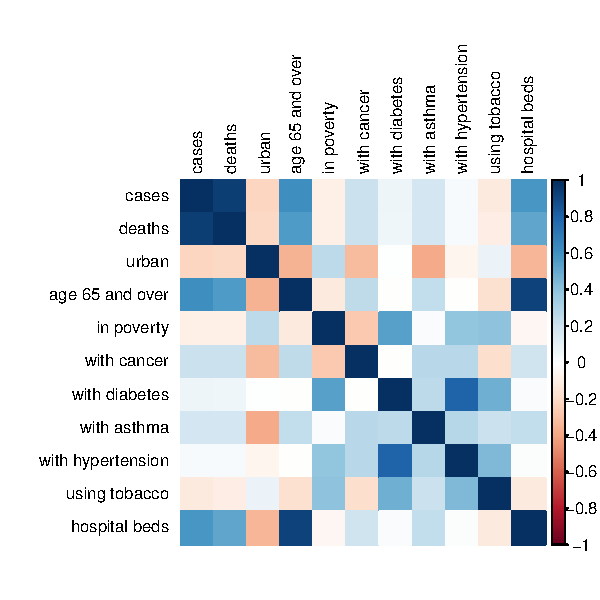
\includegraphics[width=1\linewidth]{draft_files/figure-latex/fig_corr-1} \caption{Correlation Matrix of selected U.S metrics. An example of exploratory analysis on data returned by the function `getus\_all`. Colours indicates Pearson's correlation between pairs of variables.}\label{fig:fig_corr}
\end{figure}

The main analysis of Wu et al.~\citeyearpar{wu2020m}, a zero-inflated
negative binomial mixed models, was replicated using updated U.S data
and by including an additional factor (percent of people suffering of
hypertension) in the model.

\begin{Shaded}
\begin{Highlighting}[]
\CommentTok{# remotes::install_github("nyiuab/NBZIMM")}
\CommentTok{# library(NBZIMM)}
\NormalTok{pm2}\FloatTok{.5}\NormalTok{_model <-}\StringTok{ }\KeywordTok{glmm.zinb}\NormalTok{(}
  \DataTypeTok{fixed =}
\NormalTok{    deaths }\OperatorTok{~}
\StringTok{    }\NormalTok{pm2}\FloatTok{.5} \OperatorTok{+}
\StringTok{      }\KeywordTok{scale}\NormalTok{(median_income) }\OperatorTok{+}
\StringTok{      }\KeywordTok{scale}\NormalTok{(perc_edu_somecollege) }\OperatorTok{+}
\StringTok{      }\KeywordTok{scale}\NormalTok{(perc_lat) }\OperatorTok{+}
\StringTok{      }\KeywordTok{scale}\NormalTok{(perc_black) }\OperatorTok{+}
\StringTok{      }\KeywordTok{scale}\NormalTok{(age65_over) }\OperatorTok{+}
\StringTok{      }\KeywordTok{scale}\NormalTok{(total_tests) }\OperatorTok{+}
\StringTok{      }\KeywordTok{scale}\NormalTok{(total_beds) }\OperatorTok{+}
\StringTok{      }\KeywordTok{scale}\NormalTok{(perc_obesity) }\OperatorTok{+}
\StringTok{      }\KeywordTok{scale}\NormalTok{(perc_hypertension) }\OperatorTok{+}
\StringTok{      }\KeywordTok{scale}\NormalTok{(perc_tobacco_use) }\OperatorTok{+}
\StringTok{      }\KeywordTok{scale}\NormalTok{(summer_temp) }\OperatorTok{+}
\StringTok{      }\KeywordTok{scale}\NormalTok{(winter_temp) }\OperatorTok{+}
\StringTok{      }\KeywordTok{scale}\NormalTok{(summer_hum) }\OperatorTok{+}
\StringTok{      }\KeywordTok{scale}\NormalTok{(winter_hum) }\OperatorTok{+}
\StringTok{      }\KeywordTok{offset}\NormalTok{(}\KeywordTok{log}\NormalTok{(total_pop)),}
  \DataTypeTok{random =} \OperatorTok{~}\StringTok{ }\DecValTok{1} \OperatorTok{|}\StringTok{ }\NormalTok{state,}
  \DataTypeTok{data =}\NormalTok{ us_last}
\NormalTok{)}
\end{Highlighting}
\end{Shaded}

\begin{verbatim}
## Computational iterations: 9 
## Computational time: 0.016 minutes
\end{verbatim}

Results {[}table \ref{tab:tab_coef}{]} indicates, as in Wu et
al.~\citeyearpar{wu2020m}, a significant effect of fine particulate 2.5
on COVID-19 mortality.

\begin{table}[ht]
\centering
\begin{tabular}{cccccc}
  \hline
 & Value & Std.Error & DF & t-value & p-value \\ 
  \hline
(Intercept) & -11.79 & 1.14 & 199.00 & -10.32 & 0.00 \\ 
  $\mu_g/m^3$ & 0.23 & 0.12 & 199.00 & 1.84 & 0.07 \\ 
  median income & 0.13 & 0.14 & 199.00 & 0.97 & 0.33 \\ 
  college education & -0.35 & 0.12 & 199.00 & -3.05 & 0.00 \\ 
  hispanic or latinos & 0.14 & 0.13 & 199.00 & 1.11 & 0.27 \\ 
  black or afroamerican & 0.02 & 0.16 & 199.00 & 0.14 & 0.89 \\ 
  age 65 and over & 0.34 & 0.24 & 199.00 & 1.44 & 0.15 \\ 
  number of tests & 0.46 & 0.24 & 3.00 & 1.89 & 0.16 \\ 
  hospital beds & -0.24 & 0.23 & 199.00 & -1.06 & 0.29 \\ 
  obesity & 0.19 & 0.13 & 199.00 & 1.50 & 0.14 \\ 
  hypertension & 0.53 & 0.22 & 199.00 & 2.41 & 0.02 \\ 
  tabacco use & -0.16 & 0.15 & 199.00 & -1.03 & 0.30 \\ 
  summer temperature & -0.39 & 0.43 & 199.00 & -0.91 & 0.36 \\ 
  winter temperature & -0.30 & 0.52 & 199.00 & -0.57 & 0.57 \\ 
  summer humidity & -0.11 & 0.25 & 199.00 & -0.44 & 0.66 \\ 
  winter humidity & -0.21 & 0.20 & 199.00 & -1.05 & 0.30 \\ 
   \hline
\end{tabular}
\caption{Coefficients of the model. A zero-inflated negative binomial mixed model was fitted of data of U.S counties (2020-05-10)} 
\label{tab:tab_coef}
\end{table}

\hypertarget{conclusions}{%
\section{Conclusions}\label{conclusions}}

The \texttt{R} package \texttt{covid19census} extracts and integrates
epidemiological COVID-19 data (Italy and U.S at the regional and county
level, respectively) with several other demographic and health related
indexes. Currently, the dataframes returned by the main functions
\texttt{getus\_all} and \texttt{getit\_all}, consist of 337 variables
per 3225 U.S counties, and of 64 variables per 21 Italy regions (19
regions and autonomous provinces), respectively. By combining data form
different sources, the package is aimed at promoting and simplifying the
analysis and modeling of COVID-19 data by the scientific community.


\begin{notes}[Acknowledgements]
\emph{Funding} : L.M. and C.Z were supported by NIH-NCI grants
P30CA006973, U01CA196390, R01CA200859and the Department of Defense (DoD)
office of the Congressionally Directed Medical Research Programs (CDMRP)
award W81XWH-16-1-0739.

\emph{Conflict of interest} : none.
\end{notes}


\renewcommand\refname{References}

\bibliography{mybibfile.bib}



\end{document}
